\label{Principios de Machine Learning}
\section{Principios de Machine Learning}

Este trabajo integrador se incluyen campos de la inteligencia artificial, los cuales son Visión por Computadora y Deep Learning o Aprendizaje profundo. 
Esta sección tiene el propósito de hacer una introducción teórica a ambas ramas de la inteligencia artificial.

\subsection{Introducción: Visión por Computadora}
Una de las ramas de investigación más populares y utilizada de la Inteligencia Artificial es la Visión por Computadora o también llamada Computer Vision \cite{computervision1} \cite{computervision2} \cite{computervision3}.
Este campo se centra en intentar replicar funciones del sistema de visión humano, de forma que permita a las computadoras identificar y procesar objetos en imágenes o vídeos de forma similar a como los humanos lo hacen. Tiempo atrás, la capacidad de la visión por computadora era muy limitada, pero hoy en día hay muchas tecnologías que utilizan la visión por computadora, entre las cuales se encuentran el reconocimiento de objetos, la detección de sucesos, la reconstrucción de una escena y la restauración de imágenes.

En la actualidad, muchos son los campos que se han visto beneficiados por este conjunto de técnicas. Uno de los más conocidos es el de la robótica por medio de sensores o de cámaras, siendo estos últimos dispositivos idóneos para la aplicación de las estrategias de visión por computadora.

Sin embargo, podemos destacar otros ámbitos capaces de reconocer objetos, por ejemplo, en sistemas de seguridad, seguimiento de objetos o detección de anomalías en piezas fabricadas en una cadena de producción, medicina, etc.

\subsection{Fundamentos de Machine Learning}

Machine Learning \cite{ml}, es esencialmente un conjunto de algoritmos diseñado por un ser humano, pero que aprenden de los datos a los cuales son expuesto, dicho de otra manera, un conjunto de datos se usa para entrenar un modelo matemático de modo que cuando vea datos similares en el futuro, sepa reconocerlos. Los modelos, normalmente, toman datos como entrada y luego emiten una predicción de algo de interés. Estos algoritmos son ejecutados típicamente en algún tipo de computadora especial y sirven para resolver problemas de:
\begin{itemize}
    \item \textbf{Clasificación:} Retorna probabilidades de clase o distingue clases. Figura \ref{fig:clasificacion}.
    \item \textbf{Regresión:} Hace predicciones o estimaciones (en general numéricas). Figura \ref{fig:regresion}.
\end{itemize}

\begin{figure}[h!]
    \centering
    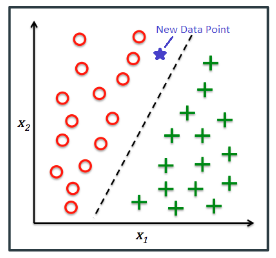
\includegraphics[width=0.5\textwidth]{img/clasificacion.png}
    \caption{Clasificación. Fuente: \cite{aprendisajesup}}
    \label{fig:clasificacion}
\end{figure}

\begin{figure}[h!]
    \centering
    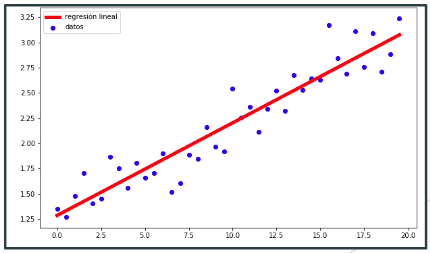
\includegraphics[width=0.8\textwidth]{img/regresion.png}
    \caption{Regresión. Fuente: \cite{aprendisajesup}}
    \label{fig:regresion}
\end{figure}

\newpage
El problema surge cuando se intenta resolver un problema de clasificación que no es linealmente separable. Aquí es donde aparecen la Redes Neuronales, con su capacidad de transformar estos problemas en linealmente separables. Figura \ref{fig:linealmente separables}.

\begin{figure}[h!]
    \centering
    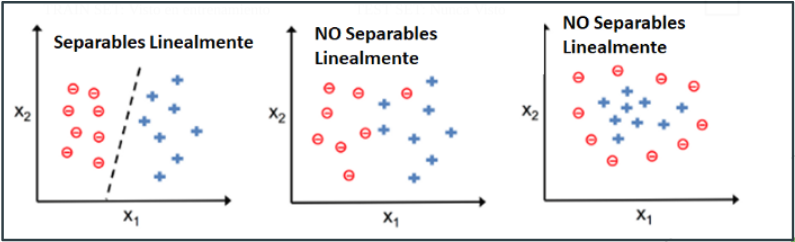
\includegraphics[width=1\textwidth]{img/linealmenteSeparable.png}
    \caption{Ejemplo Linealmente Separable. Fuente: \cite{aprendisajesup}}
    \label{fig:linealmente separables}
\end{figure}

\newpage
\paragraph{Ajuste del modelo: ¿Por qué se entrena un modelo de Machine Learning?}

Así como en la vida real a un ser humano se le enseña desde temprana edad a identificar distintos tipos de objetos dentro de su campo de visión, un modelo (o algoritmo) de Machine Learning tiene que aprender a detectar reconocer correctamente.

Para ello se lo entrena a partir de imágenes ya correctamente (ground truth) etiquetadas (bounding box) y, a grandes rasgos, si la predicción es correcta, se le alienta a seguir por ese camino y por el contrario si falla se lo alienta a ir en la dirección opuesta. Esto sería el ajuste con las perillas de una caja negra que viene a representar una abstracción de un modelo de Redes Neuronales, tal y como se representa en la siguiente Figura \ref{fig:abstraccion red neuronal}.

\begin{figure}[h]
    \centering
    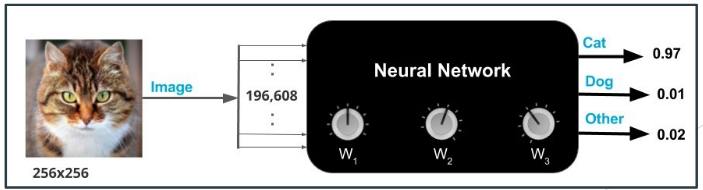
\includegraphics[width=1\textwidth]{img/RedNeuronal.png}
    \caption{Abstracción de una Red Neuronal. Fuente: \cite{redneuronalbasic}}
    \label{fig:abstraccion red neuronal}
\end{figure}

Se entrena el modelo a partir de un conjunto de datos lo suficientemente diverso, de tal manera que el modelo generalice y pueda realizar predicciones a partir de imágenes que nunca ``vio'' (analizó).

\begin{figure}[h!]
    \centering
    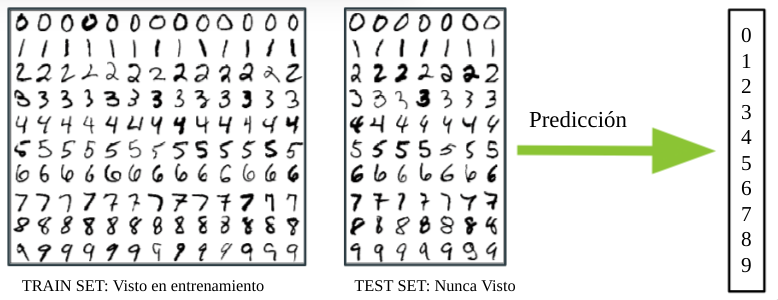
\includegraphics[width=1\textwidth]{img/RedNeuronal1.png}
    \caption{Ejemplo Machine Learning. Fuente: \cite{img_RedNeuronal1}}
    \label{fig:red neuronal 1}
\end{figure}

\subsection{Redes Neuronales}
Las Redes Neuronales Artificiales (ANNs por su siglas en inglés) son modelos matemáticos concebidos en un principio para estudiar (de cierta manera), el comportamiento del cerebro humano.
Estos modelos matemáticos son llamados Redes Neuronales porque fueron inspirados por neuronas biológicas, tal y como formalizaron: McCulloch y Pitts (1943) \cite{McCulloch1943-nf}; y Hebb & Hebb (1949) \cite{Morris1999-xd}. A grandes rasgos, se resume, que las Redes Neuronales Artificiales son formadas por circuitos neuronales y las interconexiones entre neuronas, llamadas sinapsis. Son llamadas sistemas conexionistas porque la información es codificada en los parámetros de las conexiones entre unidades.

En un principio, no hay una división clara entre conexionismo y neurociencia computacional, la principal diferencia es que los sistemas conexionistas se centran en procesos cognitivos de alto nivel, tales como: reconocimiento, memoria, comprensión  y razonamiento; en vez de detalles específicos del funcionamiento neuronal. En la década de 1980, el conexionismo experimentó una fuerte revitalización al formalizar una regla general de aprendizaje conocida como Backpropagation LeCun et al.(1988) \cite{lecun}. Backpropagation, que continua como el ``Hoyo en uno'' de la investigación conexionista contemporánea, permite a una amplia gama de modelos ANNs aprender una determinada función de mapeo de una entrada a una salida.

Hoy, el conexionismo esta mayormente englobado en el aprendizaje profundo (Deep Learning), ya que ha logrado  resultados notables en cuanto a avances en diversas aplicaciones. Aun no esta claro si las ANNs están limitadas en algún aspecto importante o no (por ejemplo, problemas de olvido catastrófico y ataques adversarios); sin embargo, está claro que los modelos de Deep Learning son lo suficientemente poderosos y flexibles para lidiar con muchos problemas.

En este capítulo, se introducen brevemente conceptos básicos relacionados al presente trabajo. Primero, se presentan las Redes Neuronales y su proceso de dos etapas (inferencia y entrenamiento). Luego, se introducen Clasificadores y otros modelos y técnicas esenciales para entender este trabajo. Finalmente, se presenta la literatura sobre Visión por Computadora y las métricas de evaluación centrales para medir la performance de los modelos de Machine Learning.

\subsection{Definición formal de Redes Neuronales}
En el aprendizaje supervisado, un dataset (conjunto de datos) de entrenamiento \mathbf{D = (xi, yi)}, representa a una función de mapeo (\mathbf{F : xi → yi}) definida por sus observaciones \textit{xi} y su correspondiente etiqueta \textit{yi}, que son variables independiente e idénticamente distribuidas (i.i.d) de una distribución \textit{Px},y. Luego, una red Neuronal es entrenada para aprender una función de mapeo \textit{f} que aproxima a \textit{F}. El objetivo de una Red Neuronal es relacionar correctamente las entradas \textit{xi} con las salidas \textit{yi}, mediante la adaptación de sus parámetros $\theta$. Por ejemplo, en un problema de clasificación de dígitos, \textit{xi} consiste en imágenes de dígitos mientras que \textit{yi} corresponde a la categoría del dígito.


En dos pasos, un clasificador de redes Neuronales aprende una función de mapeo \mathbf{y = f(x; $\theta$)} y adapta los parámetros $\theta$ que minimiza las predicciones del modelo y la verdad absoluta.

El primer paso se llama propagación Feedfoward o inferencia. La información de entrada \textit{x} fluye a través de la red Neuronal, siendo multiplicada por sus computaciones intermedias hacia la salida. En la mayoría de los casos, el mapeo \mathbf{f(x) : x → y},  es una función de activación descripta por \mathbf{f(x) : g3 ◦ g2 ◦ g1(x)} donde \textit{gl} son las capas intermedias conectadas en cadena \mathbf{y = f(x) = g3(g2(g1(x)))}. Las capas intermedias son parametrizadas por un vector de pesos \textit{$\theta$l}, que es utilizado para ponderar la entrada antes de ser transformadas por la función de activación. En cada capa oculta, la función de activación transforma la suma ponderada de las entradas en una salida. Las capas ocultas pueden también contener parámetros \textit{bias} que son utilizados usualmente para desplazar la suma ponderada de la entrada. Una capa es comúnmente representada como: \mathbf{gl(x) = φ($\theta$l, x)} donde \textit{$\theta$l} es el parámetro de la capa y \textit{φ} es la función de activación de la capa. Una red neuronal comprende de una capa de entrada \textit{g1}, que es la primer capa de la red, una capa de salida \textit{g3} y varias capas intermedias. La ultima capa, la capa de salida, es donde se espera que esté la predicción.
El largo total de esta cadena representa la profundidad del modelo y es de donde proviene el termino aprendizaje profundo (Deep Learning).

Los datos de entrenamiento provistos, comprenden de observaciones de F evaluados a diferentes puntos. Cada muestra \textit{xi} es acompañada de una etiqueta \textit{yi = F(xi)}, que representa la salida deseada para la capa de salida. En conjunto, la etiqueta especifica qué debe ser la capa de salida. Sin embargo, el comportamiento de salida de las capas intermedias no esta directamente especificado por los datos de entrenamiento, por eso se llaman capaz ocultas.

El segundo paso, es llamado entrenamiento y consiste en ``enviar hacia atrás'' (backpropagation), una señal de error sobre los parámetros del modelo (Riedmiller and Braun (1993) \cite{Riedmiller1993ADA}). Una función de pérdida (Loss function), es utilizada para computar el error cometido por el modelo en sus predicciones; esto es, la pérdida es alta cuando el modelo esta haciendo un trabajo pobre y por el contrario es baja cuando está performando bien. La señal de error, es el valor de la diferencia entre las etiquetas predichas y las verdaderas etiquetas deseadas. Luego, este valor de error, es utilizado para ajustar los parámetros del modelo para reducir la discrepancia en la predicción. El gradiente de la función de perdida con respecto a capas previas, es utilizado como la regla de actualización para ajustar los parámetros de cada capa. El proceso de aprendizaje es repetido hasta converger, por lo que un optimizador iterativamente computa el gradiente sobre lotes aleatoriamente muestreados del set de entrenamiento. Cuando una red neuronal encuentra un set de parámetros ``óptimo'', está lista para ser desplegada y comenzar así, a hacer predicciones sobre ejemplos nunca antes observados.

Un amplio rango de características (features), permiten a las ANNs, enseñarle a \textit{f} a encontrar un mapeo válido entre las entradas y las salidas. Por ejemplo, para evadir limitaciones lineales, funciones no lineales $\Psi$ son utilizadas en capas ocultas en vez de transformaciones lineales, ya que provee mayores grados de libertad, que habilitan al modelo a ``entender'' las relaciones no lineales entre los ejemplos \textit{x} y sus correspondientes etiquetas \textit{y}. Las transformaciones no lineales, permiten transformar problemas no linealmente separables en linealmente separables. Más específicamente, las funciones no lineales, permiten al espacio de entrada ser doblado, por lo que éste espacio puede ser dividido en regiones lineales más pequeñas (Pascanu et al.(2013) \cite{pmlr-v28-pascanu13}). La transformación no lineal, la correcta función de perdida y un apropiado número de parámetros en las capas ocultas, permiten a la red neuronal, aproximar cualquier función de mapeo. Éste es el origen del término aproximado universal (Hornik et al. (1989)). Para una introducción detallada de Redes Neuronales, por favor referirse a Hornik et al. (1989) \cite{HORNIK1989359}.

La función de mapeo aprendida \textit{f($\theta$, x)}, es actualizada y evaluada todo el tiempo en aprendizaje continuo. Cuando se evalúa la performance de un clasificador, lo que es juzgado detrás de escena, es el grado de degradación de la función de mapeo relativa a la función original de mapeo F.
